\begin{frame}
	\frametitle{Nivel de di\'agnostico}
	
	\begin{columns}[T] % contents are top vertically aligned
		\begin{column}[T]{5cm} % each column can also be its own environment
			\begin{itemize}
				\item Usando distintos m\'etodos de diagn\'ostico
				\begin{itemize}
					\item \textit{Clustering}
					\item Clasificaci\'on supervisada
					\item ...
				\end{itemize}
			\end{itemize}
		\end{column}
		\begin{column}[T]{5cm} % alternative top-align that's better for 
		%graphics
			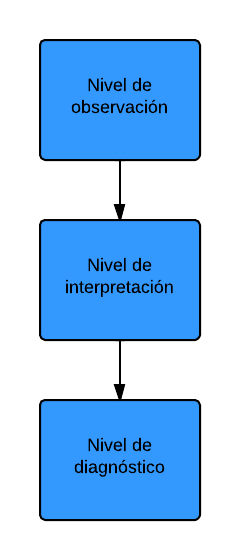
\includegraphics[width=0.5\linewidth]{./Figures/NivelDeDiagnostico.png}
		\end{column}
	\end{columns}
\end{frame}